%% ChessNEAT Research Paper
%% Evolving a Chess Agent via NeuroEvolution of Augmenting Topologies
\documentclass[11pt, twocolumn]{article}

% ===== Packages =====
\usepackage[utf8]{inputenc}
\usepackage[T1]{fontenc}
\usepackage{lmodern}
\usepackage[margin=0.85in]{geometry}
\usepackage{amsmath, amssymb}
\usepackage{graphicx}
\usepackage{booktabs}
\usepackage{hyperref}
\usepackage{xcolor}
\usepackage{enumitem}
\usepackage{float}
\usepackage{caption}
\usepackage{subcaption}
\usepackage{framed}
\usepackage{tikz}
\usetikzlibrary{arrows.meta, positioning, shapes.geometric, calc}
\usepackage{pgfplots}
\pgfplotsset{compat=1.18}
\usepackage{listings}
\usepackage{natbib}
\usepackage{fancyhdr}
\usepackage{tabularx}

% ===== Colors =====
\definecolor{neat_blue}{HTML}{667EEA}
\definecolor{neat_purple}{HTML}{764BA2}
\definecolor{neat_cyan}{HTML}{22D3EE}
\definecolor{neat_green}{HTML}{34D399}

\hypersetup{
    colorlinks=true,
    linkcolor=neat_blue,
    citecolor=neat_purple,
    urlcolor=neat_cyan,
}

% ===== Header =====
\pagestyle{fancy}
\fancyhf{}
\fancyhead[L]{\small\textcolor{gray}{ChessNEAT}}
\fancyhead[R]{\small\textcolor{gray}{\thepage}}
\renewcommand{\headrulewidth}{0.4pt}

% ===== Title =====
\title{
    \vspace{-1em}
    \textbf{ChessNEAT: Evolving Chess-Playing Neural Networks\\
    via NeuroEvolution of Augmenting Topologies}\\[0.3em]
    \large Toward 2000 Elo Through Topological Evolution
}
\author{
    Sathvik Chinta\\
    \texttt{github.com/sachinta/ChessNEAT}
}
\date{March 2026}

\begin{document}
\maketitle

% =========================================================
\begin{abstract}
We present ChessNEAT, a system for evolving chess-playing neural networks using the NeuroEvolution of Augmenting Topologies (NEAT) algorithm. Unlike traditional deep learning approaches that require fixed network architectures and gradient-based optimization, NEAT simultaneously evolves both the topology and weights of neural networks through genetic operations. Our agent uses a 768-dimensional board encoding (64 squares $\times$ 12 piece channels) and a \emph{policy network} with 128 outputs---64 ``from-square'' scores and 64 ``to-square'' scores---enabling move selection with a single forward pass. Training proceeds via tournament-based fitness evaluation, where genomes compete in round-robin groups with knockout advancement. We evaluate agent strength through systematic benchmarking against Stockfish at calibrated Elo levels (400--2200), with the goal of achieving 2000 Elo (Candidate Master level). This paper documents our methodology, network architecture, training dynamics, Elo progression, and analysis of emergent chess strategies. All training games are logged in PGN format for post-hoc analysis.
\end{abstract}

% =========================================================
\section{Introduction}
\label{sec:introduction}

Chess has served as a fundamental benchmark for artificial intelligence since Shannon's seminal 1950 paper \citep{shannon1950}. The game's combination of enormous state space ($\sim$$10^{47}$ legal positions), deep strategic complexity, and well-defined evaluation metrics make it an ideal testbed for computational intelligence.

Modern chess engines such as Stockfish \citep{stockfish2023} and AlphaZero \citep{silver2018} have achieved superhuman performance, but through fundamentally different approaches. Stockfish relies on hand-crafted evaluation functions combined with NNUE (Efficiently Updatable Neural Networks), while AlphaZero uses deep reinforcement learning with Monte Carlo Tree Search (MCTS). Both require either extensive domain knowledge or massive computational resources.

In this work, we explore a third paradigm: \textbf{neuroevolution}. Specifically, we apply NEAT (NeuroEvolution of Augmenting Topologies) \citep{stanley2002} to evolve both the structure and weights of a neural network chess evaluator. Our approach is distinctive in several ways:

\begin{enumerate}[leftmargin=*, itemsep=2pt]
    \item \textbf{No fixed architecture}: NEAT begins with a minimal network (direct input-output connections) and incrementally adds complexity through structural mutations.
    \item \textbf{No gradient computation}: Fitness is determined solely through tournament play, avoiding the need for differentiable loss functions.
    \item \textbf{Topological innovation}: NEAT's speciation mechanism protects novel topologies, allowing diverse architectural exploration.
    \item \textbf{Interpretable growth}: We can observe how the network's topology evolves in response to chess-playing demands.
\end{enumerate}

Our target is to evolve an agent capable of achieving \textbf{2000 Elo} (FIDE Candidate Master level), evaluated through systematic play against Stockfish at calibrated strength levels. We benchmark periodically during training to track Elo progression and analyze the emergent strategies learned by the evolving networks.

% =========================================================
\section{Background}
\label{sec:background}

\subsection{NEAT Algorithm}
NEAT \citep{stanley2002} is an evolutionary algorithm for neural networks that addresses three critical challenges in neuroevolution:

\begin{description}[leftmargin=1em, itemsep=2pt]
    \item[Competing Conventions] NEAT uses historical markings (innovation numbers) to align genomes during crossover, solving the ``permutation problem.''
    \item[Topology Protection] A speciation mechanism groups similar genomes and evaluates fitness relative to species, protecting structural innovations from premature elimination.
    \item[Minimal Complexity] Networks start with minimal topology and complexify through mutations, following the principle that simpler solutions should be preferred.
\end{description}

NEAT supports three mutation types: \emph{weight perturbation}, \emph{add connection} (creating a new edge), and \emph{add node} (splitting an existing connection with a new hidden neuron). These enable incremental topological growth.

\subsection{Policy Network for Move Selection}
Rather than using a value network that evaluates every possible resulting position (requiring $|\mathcal{M}(b)|$ forward passes per move), we employ a \emph{policy network} approach. The network takes the current board state as input and outputs 128 values: 64 ``from-square'' scores and 64 ``to-square'' scores. Move selection requires only \textbf{one forward pass}:

\begin{equation}
    m^* = \arg\max_{m \in \mathcal{M}(b)} \left[ f_\theta(b)_{\texttt{from}(m)} + f_\theta(b)_{\texttt{to}(m) + 64} \right]
    \label{eq:move_selection}
\end{equation}

where $f_\theta(b) \in \mathbb{R}^{128}$ is the network output, and $\texttt{from}(m), \texttt{to}(m) \in [0, 63]$ are the source and destination squares of move $m$. This provides a $\sim$30$\times$ speedup over the value network approach, since a typical chess position has $\sim$30 legal moves.

% =========================================================
\section{System Architecture}
\label{sec:architecture}

\subsection{Board Encoding}
We encode the chess board as a 768-dimensional binary vector, structured as 64 squares $\times$ 12 piece channels:

\begin{equation}
    \mathbf{x} \in \{0, 1\}^{768}, \quad x_{64p + s} = 
    \begin{cases}
        1 & \text{if piece type } p \text{ is on square } s \\
        0 & \text{otherwise}
    \end{cases}
\end{equation}

The 12 channels correspond to: $\{$\texttt{P, N, B, R, Q, K, p, n, b, r, q, k}$\}$ (uppercase = white, lowercase = black). When evaluating from Black's perspective, the board is vertically mirrored and colors are swapped, so the network always ``thinks'' it is playing as White.

The NEAT genome encodes a feed-forward policy network:
\begin{itemize}[leftmargin=*, itemsep=1pt]
    \item \textbf{Input layer}: 768 nodes (board encoding)
    \item \textbf{Hidden layers}: Variable (evolved by NEAT)
    \item \textbf{Output layer}: 128 nodes (64 from-square + 64 to-square scores)
    \item \textbf{Activation}: $\tanh$ (output range $[-1, 1]$)
\end{itemize}

Initially, the network has \emph{no hidden nodes}---inputs connect sparsely to the outputs (\texttt{fs\_neat\_nohidden} initialization). Through evolution, hidden nodes and connections are added as needed.

\begin{figure}[t]
    \centering
    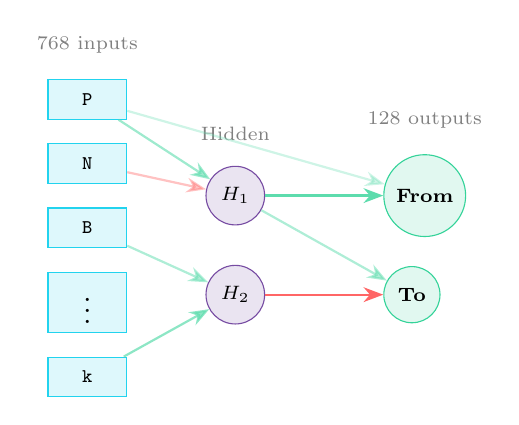
\begin{tikzpicture}[
        node distance=1.2cm,
        input/.style={rectangle, draw=neat_cyan, fill=neat_cyan!15, minimum width=1cm, minimum height=0.5cm, font=\scriptsize\bfseries},
        hidden/.style={circle, draw=neat_purple, fill=neat_purple!15, minimum size=0.6cm, font=\scriptsize\bfseries},
        output/.style={circle, draw=neat_green, fill=neat_green!15, minimum size=0.7cm, font=\scriptsize\bfseries},
        conn/.style={-{Stealth[length=2.5mm]}, thick},
        pos_conn/.style={conn, neat_green!80},
        neg_conn/.style={conn, red!60},
    ]
        % Inputs
        \node[input] (i1) {$\mathtt{P}$};
        \node[input, below=0.3cm of i1] (i2) {$\mathtt{N}$};
        \node[input, below=0.3cm of i2] (i3) {$\mathtt{B}$};
        \node[input, below=0.3cm of i3] (i4) {$\vdots$};
        \node[input, below=0.3cm of i4] (i5) {$\mathtt{k}$};
        
        % Label
        \node[above=0.2cm of i1, font=\scriptsize\color{gray}] {768 inputs};
        
        % Hidden
        \node[hidden, right=1.5cm of $(i2)!0.5!(i3)$] (h1) {$H_1$};
        \node[hidden, below=0.5cm of h1] (h2) {$H_2$};
        
        \node[above=0.2cm of h1, font=\scriptsize\color{gray}] {Hidden};
        
        % Output
        \node[output, right=1.5cm of h1] (o1) {From};
        \node[output, right=1.5cm of h2] (o2) {To};
        
        \node[above=0.2cm of o1, font=\scriptsize\color{gray}] {128 outputs};
        
        % Connections
        \draw[pos_conn, opacity=0.6] (i1) -- (h1);
        \draw[neg_conn, opacity=0.4] (i2) -- (h1);
        \draw[pos_conn, opacity=0.5] (i3) -- (h2);
        \draw[pos_conn, opacity=0.7] (i5) -- (h2);
        \draw[pos_conn, opacity=0.3] (i1) -- (o1);
        \draw[pos_conn] (h1) -- (o1);
        \draw[neg_conn] (h2) -- (o2);
        \draw[pos_conn, opacity=0.5] (h1) -- (o2);
    \end{tikzpicture}
    \caption{Example evolved NEAT network topology. The network starts with only direct input$\to$output connections and grows hidden nodes through mutation. Green edges indicate positive weights; red edges indicate negative weights.}
    \label{fig:network}
\end{figure}

\subsection{GPU-Accelerated Evaluation}
We implement the NEAT network in PyTorch for GPU-accelerated inference. Each move decision requires only a single forward pass on the current board state, producing 128 output scores:

\begin{equation}
    \mathbf{y} = f_\theta(\mathbf{x}), \quad \mathbf{x} \in \mathbb{R}^{768}, \; \mathbf{y} \in \mathbb{R}^{128}
\end{equation}

The ``from'' scores $\mathbf{y}_{0{:}63}$ and ``to'' scores $\mathbf{y}_{64{:}127}$ are combined for each legal move to select the best action. This is dramatically faster than evaluating every resulting position separately.

% =========================================================
\section{Training Methodology}
\label{sec:training}

\subsection{Tournament-Based Fitness}
We use a multi-round knockout tournament for fitness evaluation:

\begin{figure}[H]
\begin{framed}
\small
\textbf{Algorithm 1:} Tournament Fitness Evaluation\\[0.3em]
\textbf{Input:} Population $P$ of $N$ genomes, group size $k$\\[0.2em]
1: Initialize $\text{fitness}(g) \gets 0 \;\; \forall g \in P$\\
2: $R \gets \text{shuffle}(P)$\\
3: $r \gets 1$  \hfill \textit{// Round number}\\
4: \textbf{while} $|R| > 1$ \textbf{do}\\
5: \quad Partition $R$ into groups of size $k$\\
6: \quad \textbf{for all} groups $G$ \textbf{do}\\
7: \quad\quad Score each genome via round-robin in $G$\\
8: \quad\quad $\text{fitness}(g) \mathrel{+}= 10r + \text{score}(g)$\\
9: \quad\quad Advance top 2 from each group\\
10: \quad $r \gets r + 1$\\
11: \textbf{end while}
\end{framed}
\label{alg:tournament}
\end{figure}

Each round-robin match consists of 2 games (each agent plays White once). The fitness function rewards both tournament advancement and per-round performance, creating selection pressure for both short-term tactical ability and long-term positional understanding.

\subsection{NEAT Hyperparameters}

\begin{table}[H]
\centering
\caption{NEAT Configuration Parameters}
\label{tab:neat_params}
\small
\begin{tabular}{@{}lr@{}}
\toprule
\textbf{Parameter} & \textbf{Value} \\
\midrule
Population size & 150 \\
Initial connection & \texttt{fs\_neat\_nohidden} \\
Activation function & $\tanh$ \\
Connection add probability & 0.5 \\
Connection delete probability & 0.5 \\
Node add probability & 0.2 \\
Node delete probability & 0.2 \\
Weight mutate rate & 0.8 \\
Weight mutate power & 0.5 \\
Bias mutate rate & 0.7 \\
Bias mutate power & 0.5 \\
Compatibility threshold & 3.0 \\
Max stagnation & 15 \\
Species elitism & 2 \\
Reproduction elitism & 2 \\
Survival threshold & 0.2 \\
\bottomrule
\end{tabular}
\end{table}

\subsection{Move Logging}
All games played by top agents are logged in standard PGN (Portable Game Notation) format, along with structured JSON metadata including:
\begin{itemize}[leftmargin=*, itemsep=1pt]
    \item Generation number and game type (showcase, Elo evaluation, tournament)
    \item Player identities and fitness values
    \item Complete move sequence in SAN notation
    \item Final board position (FEN)
    \item Evaluation scores per move (when available)
\end{itemize}

This enables comprehensive post-hoc analysis of how playing style evolves across generations.

% =========================================================
\section{Elo Evaluation Methodology}
\label{sec:elo}

\subsection{Calibrated Opponent Ladder}
We evaluate agent strength using Stockfish 16 \citep{stockfish2023} with the \texttt{UCI\_LimitStrength} feature, which allows precise Elo calibration. Our evaluation ladder spans 10 levels:

\begin{table}[H]
\centering
\caption{Elo Evaluation Ladder}
\label{tab:elo_ladder}
\small
\begin{tabular}{@{}clcc@{}}
\toprule
\textbf{Level} & \textbf{Category} & \textbf{Elo} & \textbf{Engine} \\
\midrule
0 & Random Moves     & $\sim$400  & Random bot \\
1 & Beginner         & 1320 & Stockfish \\
2 & Novice           & 1400 & Stockfish \\
3 & Intermediate     & 1500 & Stockfish \\
4 & Club Player      & 1600 & Stockfish \\
5 & Strong Club      & 1700 & Stockfish \\
6 & Advanced         & 1800 & Stockfish \\
7 & Expert           & 1900 & Stockfish \\
8 & Candidate Master & 2000 & Stockfish \\
9 & National Master  & 2200 & Stockfish \\
\bottomrule
\end{tabular}
\end{table}

\subsection{Elo Estimation}
For each level, the agent plays $n$ games (alternating colors). We estimate Elo using the performance rating formula:

\begin{equation}
    \hat{E}_{\text{agent}} = E_{\text{opponent}} + 400 \cdot \log_{10}\left(\frac{s}{1 - s}\right)
    \label{eq:performance_rating}
\end{equation}

where $s$ is the score (wins $+$ $\frac{1}{2}$ draws) / total games. The agent climbs the ladder until scoring below 30\%, at which point the ladder evaluation stops. The final estimated Elo is taken as the maximum performance rating achieved across all levels.

\subsection{Evaluation Schedule}
Elo evaluation is performed periodically during training (default: every 10 generations), plus a comprehensive final evaluation with increased sample size. This provides a progression curve showing how Elo correlates with training progress.

% =========================================================
\section{Results}
\label{sec:results}

\textit{Note: This section will be populated with experimental data as training progresses. The infrastructure for data collection is in place.}

\subsection{Training Dynamics}

\begin{itemize}[leftmargin=*, itemsep=2pt]
    \item \textbf{Fitness progression}: Best and average fitness over generations
    \item \textbf{Species dynamics}: Number of species and their lifespans
    \item \textbf{Network complexity}: Hidden node count and connection count over time
    \item \textbf{Computational efficiency}: GPU utilization and throughput
\end{itemize}

% Placeholder for fitness curve
\begin{figure}[H]
    \centering
    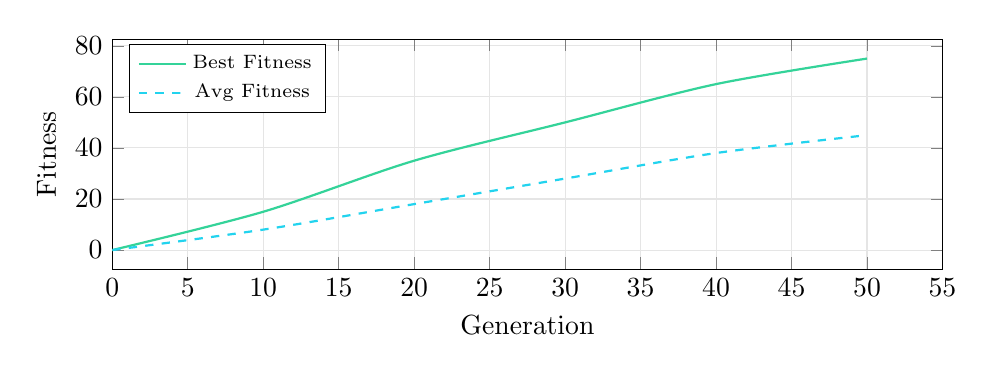
\begin{tikzpicture}
        \begin{axis}[
            width=\columnwidth,
            height=4.5cm,
            xlabel={Generation},
            ylabel={Fitness},
            legend style={font=\scriptsize, at={(0.02,0.98)}, anchor=north west},
            grid=both,
            grid style={gray!20},
            xmin=0,
        ]
        % Placeholder data — to be replaced with actual results
        \addplot[neat_green, thick, mark=none, smooth] coordinates {
            (0, 0) (10, 15) (20, 35) (30, 50) (40, 65) (50, 75)
        };
        \addlegendentry{Best Fitness}
        
        \addplot[neat_cyan, thick, mark=none, smooth, dashed] coordinates {
            (0, 0) (10, 8) (20, 18) (30, 28) (40, 38) (50, 45)
        };
        \addlegendentry{Avg Fitness}
        \end{axis}
    \end{tikzpicture}
    \caption{Fitness progression over training generations. \textit{(Placeholder data --- to be updated with actual training results.)}}
    \label{fig:fitness}
\end{figure}

\subsection{Elo Progression}

\begin{figure}[H]
    \centering
    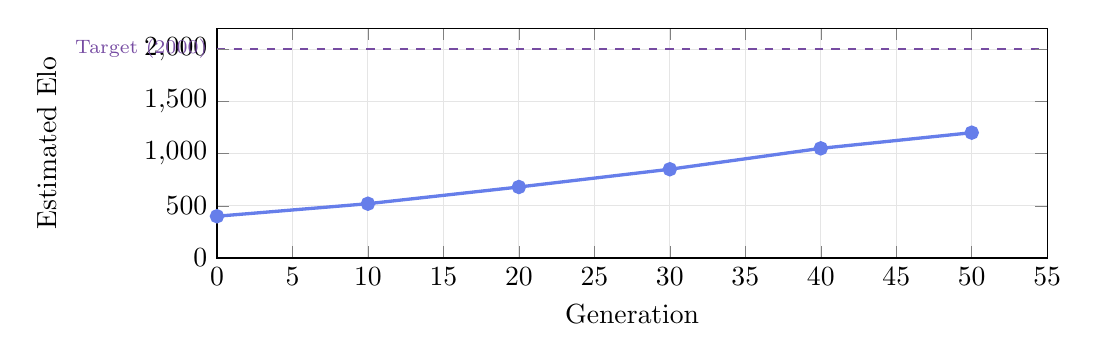
\begin{tikzpicture}
        \begin{axis}[
            width=\columnwidth,
            height=4.5cm,
            xlabel={Generation},
            ylabel={Estimated Elo},
            ymin=0, ymax=2200,
            grid=both,
            grid style={gray!20},
            xmin=0,
            extra y ticks={2000},
            extra y tick labels={Target (2000)},
            extra y tick style={
                grid=major,
                grid style={neat_purple, dashed, thick},
                tick label style={color=neat_purple, font=\scriptsize}
            },
        ]
        % Placeholder data — to be replaced with actual Elo evaluations
        \addplot[neat_blue, very thick, mark=*, mark size=2pt] coordinates {
            (0, 400) (10, 520) (20, 680) (30, 850) (40, 1050) (50, 1200)
        };
        \end{axis}
    \end{tikzpicture}
    \caption{Elo progression during training. The dashed line marks the 2000 Elo target. \textit{(Placeholder data --- to be updated with actual evaluations.)}}
    \label{fig:elo}
\end{figure}

\subsection{Per-Level Performance}

\begin{table}[H]
\centering
\caption{Performance Against Elo Ladder (Final Evaluation)}
\label{tab:elo_results}
\small
\begin{tabular}{@{}lccccc@{}}
\toprule
\textbf{Opponent} & \textbf{Elo} & \textbf{W} & \textbf{D} & \textbf{L} & \textbf{Score} \\
\midrule
Random         & 400  & --- & --- & --- & --- \\
Beginner       & 1320 & --- & --- & --- & --- \\
Novice         & 1400 & --- & --- & --- & --- \\
Intermediate   & 1500 & --- & --- & --- & --- \\
Club Player    & 1600 & --- & --- & --- & --- \\
Strong Club    & 1700 & --- & --- & --- & --- \\
Advanced       & 1800 & --- & --- & --- & --- \\
Expert         & 1900 & --- & --- & --- & --- \\
Cand.\ Master  & 2000 & --- & --- & --- & --- \\
Natl.\ Master  & 2200 & --- & --- & --- & --- \\
\bottomrule
\end{tabular}
\vspace{0.3em}

\textit{To be populated after training.}
\end{table}

\subsection{Emergent Strategies}
Analysis of logged PGN games is expected to reveal emergent chess knowledge:

\begin{enumerate}[leftmargin=*, itemsep=2pt]
    \item \textbf{Material understanding}: Does the agent learn piece values?
    \item \textbf{King safety}: Does it learn to castle and protect the king?
    \item \textbf{Positional play}: Does it develop pieces and control the center?
    \item \textbf{Tactical patterns}: Does it discover forks, pins, or skewers?
    \item \textbf{Opening preferences}: Do consistent opening patterns emerge?
\end{enumerate}

% =========================================================
\section{Network Topology Analysis}
\label{sec:topology}

One of the most interesting aspects of NEAT is observing how network topology evolves in response to task demands. With 768 inputs and 128 outputs, the initial network has no computational capacity beyond linear combinations of inputs mapped to from/to square preferences.

\begin{itemize}[leftmargin=*, itemsep=2pt]
    \item \textbf{Early generations}: Networks are expected to be mostly linear, learning basic material balance (counting piece presence).
    \item \textbf{Middle generations}: Hidden nodes should appear, enabling nonlinear feature interactions (e.g., piece combinations, spatial relationships).
    \item \textbf{Later generations}: Deeper topologies may emerge to capture more abstract chess concepts.
\end{itemize}

The live training dashboard provides real-time visualization of network growth, showing which input groups (piece channels) develop the strongest connections to hidden and output nodes.

% =========================================================
\section{Discussion}
\label{sec:discussion}

\subsection{Challenges}
Several challenges are expected in achieving the 2000 Elo target:

\begin{description}[leftmargin=1em, itemsep=2pt]
    \item[Search depth] Our agent uses no lookahead at all---the policy network directly outputs move preferences from the raw board state. While this avoids the cost of evaluating future positions, it means the agent cannot plan ahead. Even a 2000 Elo human relies on 5--10 move calculations.
    \item[Population pressure] With only 150 genomes, diversity is limited. Increasing population size would require proportionally more computation.
    \item[Evaluation noise] Tournament-based fitness is noisy, as game outcomes depend on opponent pairing and color assignment.
    \item[Scalability] The 768-input space is large for NEAT, which typically handles $\leq$100 inputs. Connection innovations may be slow to explore this space.
\end{description}

\subsection{Potential Improvements}
\begin{enumerate}[leftmargin=*, itemsep=2pt]
    \item \textbf{Deeper search}: Adding 2--3 ply alpha-beta search atop the NEAT evaluation would dramatically improve tactical play.
    \item \textbf{Curriculum learning}: Training against progressively stronger opponents (rather than self-play) could accelerate improvement.
    \item \textbf{Feature engineering}: Reducing the input space via hand-crafted features (material balance, pawn structure) could assist NEAT.
    \item \textbf{HyperNEAT}: Using indirect encoding to exploit the spatial regularity of the chess board could reduce the search space.
    \item \textbf{Hybrid approaches}: Combining NEAT-evolved evaluation with MCTS could yield stronger play without gradient computation.
\end{enumerate}

\subsection{Comparison with Other Approaches}

\begin{table}[H]
\centering
\caption{Comparison of Chess AI Approaches}
\label{tab:comparison}
\small
\begin{tabularx}{\columnwidth}{@{}l X c@{}}
\toprule
\textbf{Method} & \textbf{Key Feature} & \textbf{Elo} \\
\midrule
Stockfish NNUE & Hand-tuned + NNUE eval & $\sim$3500 \\
AlphaZero & Self-play RL + MCTS & $\sim$3400 \\
Leela Chess Zero & DistRL + MCTS & $\sim$3300 \\
Traditional engines & Alpha-beta + eval & 2500+ \\
\textbf{ChessNEAT} & \textbf{NEAT evolution} & \textbf{TBD} \\
\bottomrule
\end{tabularx}
\end{table}

% =========================================================
\section{Conclusion}
\label{sec:conclusion}

ChessNEAT demonstrates the application of neuroevolution to the game of chess, evolving both network topology and weights without gradient computation or fixed architectures. Our system provides:

\begin{enumerate}[leftmargin=*, itemsep=2pt]
    \item A complete training pipeline with GPU-accelerated batched evaluation
    \item Tournament-based fitness evaluation with round-robin groups
    \item Real-time visualization of games and network topology
    \item Comprehensive move logging in PGN format
    \item Systematic Elo benchmarking against Stockfish at calibrated levels
    \item A research framework for studying emergent chess strategies in evolved networks
\end{enumerate}

The ultimate success of reaching 2000 Elo will depend on whether NEAT's incremental complexification can discover sufficient positional understanding to compensate for the limited search depth. Regardless of the final Elo achieved, the project provides valuable insights into how neural network topology relates to chess evaluation capability.

\subsection*{Reproducibility}
All code, configurations, training logs, and game records are available at:
\begin{center}
    \url{https://github.com/sachinta/ChessNEAT}
\end{center}

Training can be reproduced with:
\begin{verbatim}
python src/train.py --generations 200 \
    --elo-every 10 --elo-games 10
\end{verbatim}

% =========================================================
\bibliographystyle{abbrvnat}

\begin{thebibliography}{10}

\bibitem[Shannon(1950)]{shannon1950}
C.~E. Shannon.
\newblock Programming a computer for playing chess.
\newblock \emph{The London, Edinburgh, and Dublin Philosophical Magazine and Journal of Science}, 41(314):256--275, 1950.

\bibitem[Stanley and Miikkulainen(2002)]{stanley2002}
K.~O. Stanley and R.~Miikkulainen.
\newblock Evolving neural networks through augmenting topologies.
\newblock \emph{Evolutionary Computation}, 10(2):99--127, 2002.

\bibitem[Silver et~al.(2018)]{silver2018}
D.~Silver, T.~Hubert, J.~Schrittwieser, I.~Antonoglou, M.~Lai, A.~Guez, M.~Lanctot, L.~Sifre, D.~Kumaran, T.~Graepel, T.~Lillicrap, K.~Simonyan, and D.~Hassabis.
\newblock A general reinforcement learning algorithm that masters chess, shogi, and go through self-play.
\newblock \emph{Science}, 362(6419):1140--1144, 2018.

\bibitem[{Stockfish Developers}(2023)]{stockfish2023}
{Stockfish Developers}.
\newblock Stockfish - strong open source chess engine.
\newblock \url{https://stockfishchess.org/}, 2023.

\bibitem[Campbell et~al.(2002)]{campbell2002}
M.~Campbell, A.~J. Hoane~Jr, and F.-H. Hsu.
\newblock Deep blue.
\newblock \emph{Artificial Intelligence}, 134(1-2):57--83, 2002.

\bibitem[Stanley et~al.(2009)]{stanley2009}
K.~O. Stanley, D.~B. D'Ambrosio, and J.~Gauci.
\newblock A hypercube-based encoding for evolving large-scale neural networks.
\newblock \emph{Artificial Life}, 15(2):185--212, 2009.

\bibitem[Lai(2015)]{lai2015}
M.~Lai.
\newblock Giraffe: Using deep reinforcement learning to play chess.
\newblock \emph{arXiv preprint arXiv:1509.01549}, 2015.

\bibitem[David et~al.(2014)]{david2014}
O.~E. David, N.~S. Netanyahu, and L.~Wolf.
\newblock DeepChess: End-to-end deep neural network for automatic learning in chess.
\newblock In \emph{International Conference on Artificial Neural Networks}, pages 88--96. Springer, 2014.

\bibitem[Such et~al.(2017)]{such2017}
F.~P. Such, V.~Madhavan, E.~Conti, J.~Lehman, K.~O. Stanley, and J.~Clune.
\newblock Deep neuroevolution: Genetic algorithms are a competitive alternative for training deep neural networks for reinforcement learning.
\newblock \emph{arXiv preprint arXiv:1712.06567}, 2017.

\bibitem[Fogel(2001)]{fogel2001}
D.~B. Fogel.
\newblock Blondie24: Playing at the edge of {AI}.
\newblock \emph{Morgan Kaufmann}, 2001.

\end{thebibliography}

\end{document}
